\chapter{Model-Learning Framework}
\label{ch:methodology} %TODO Update chapter title? e.g., The Model-Learning Framework

Our interest in this thesis lies in the development of probabilistic models for systems whose dynamics are stochastic.
The objective is to use a dataset of execution traces of a system to attain an accurate system representation, which can be used to obtain plans for optimal automated control of the system under consideration.
In this chapter we describe our proposed framework that applies learning algorithms to obtain probabilistic models in the form of \acrshortpl{acr:mdp} and optimizes for a performance-maximizing model by sampling multiple hyper-parameter settings for these learning algorithms.

In \autoref{sec:model-learning-routine} a detailed explanation is provided of the learning and optimization routine which forms the basis of our framework.

\section{Model Learning and Optimization Routine}
\label{sec:model-learning-routine}

As the development of probabilistic models oft to be a difficult an time-costly process for a human designer, an appealing idea is to automate the model development process by applying learning algorithms on a dataset of execution traces of the system under consideration.
However, to achieve effective planning in a real-world environment, the models that are learned should accurately reflect the dynamics of the system.

There are two major reasons for a learned model to not yield good performance.
First of all, the learned model may be too complicated for the amount of available data, which leads to model over-fitting.
On the other hand, one could acquire a model that is too simple to explain the available data and so does not accurately reflect the underlying system in that situation.
Therefore, the parameters of the learning algorithm should be properly adjusted in order to acquire accurate probabilistic models.
The learning routine described in this section aims to achieve this by posing the adjustment of these parameters as an optimization task, with the objective of obtaining an \acrshort{acr:mdp} model that maximizes the performance of executing the plans that are derived from it.

\begin{figure}[!h]%[t]
	\centering
	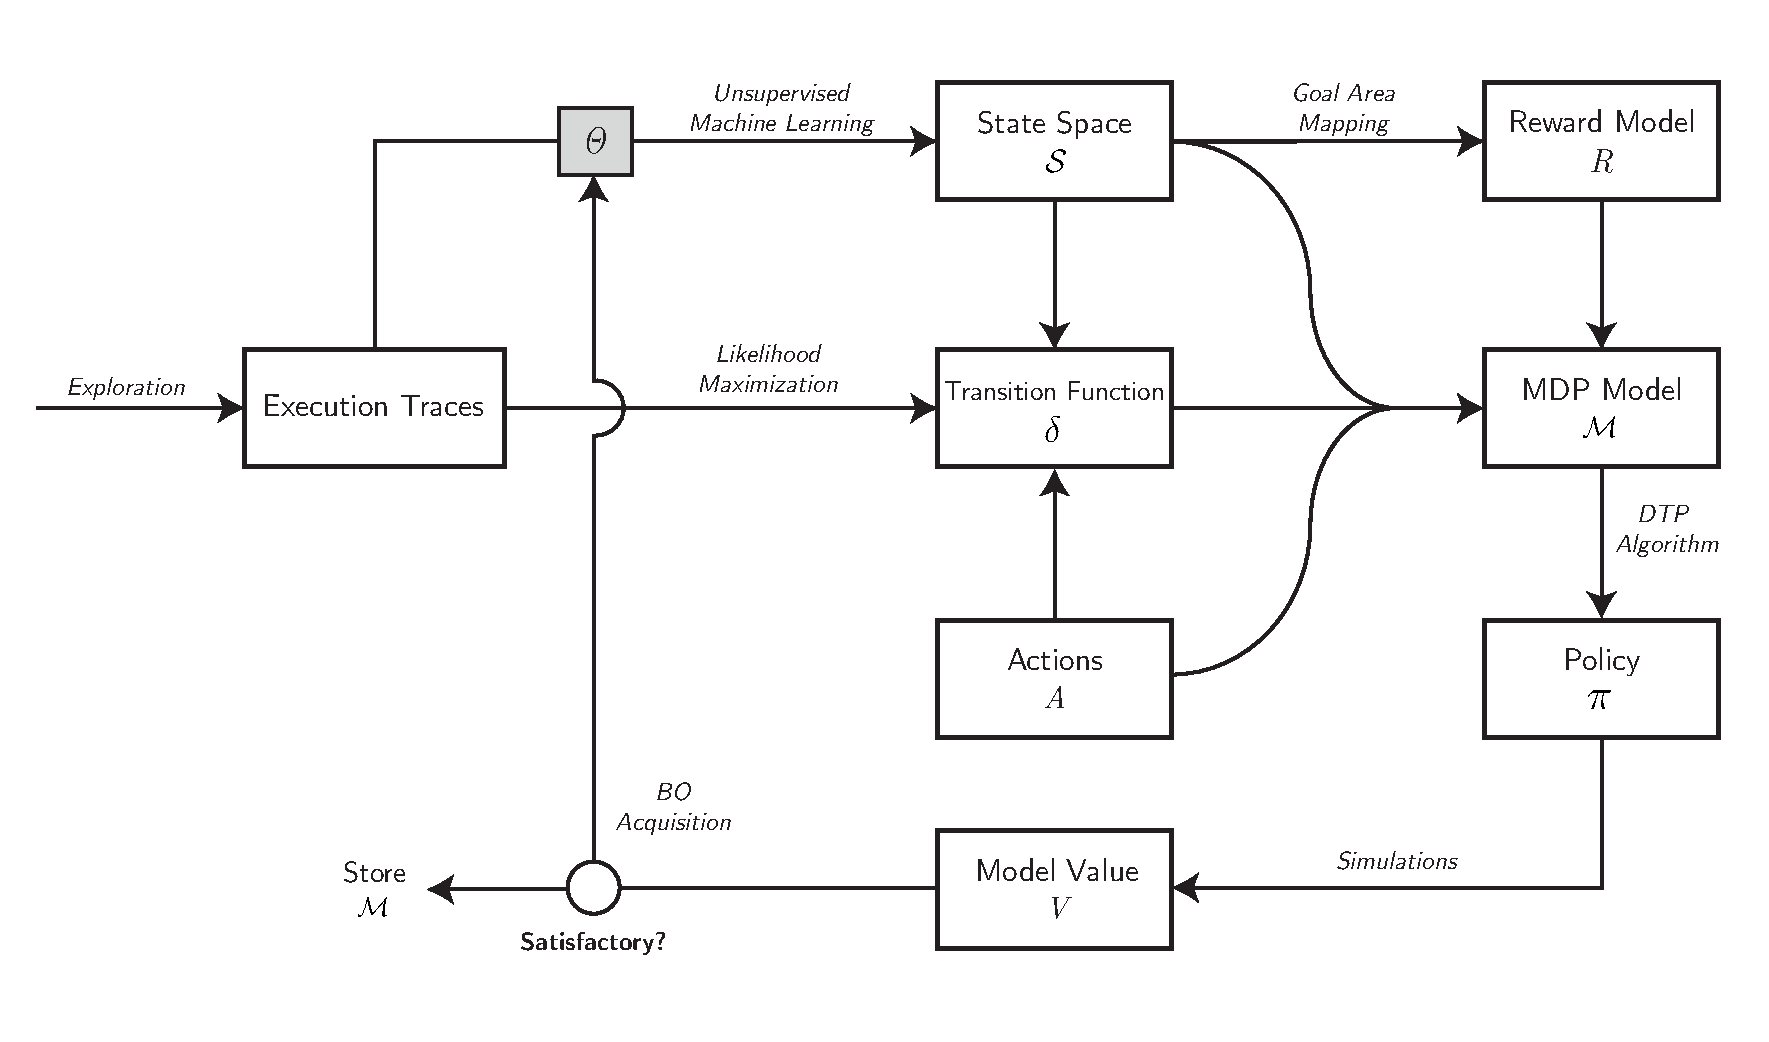
\includegraphics[width=\textwidth]{learning-cycle-complete-v2}
	\caption{Diagram of the Model Learning and Optimization Routine}
	\label{fig:learning-routine-complete}
\end{figure}

\subsection{Learning Step}
\label{sec:routine-description}

\begin{itemize}
	\item Start off with data-set of execution traces obtained beforehand
	\item A number of parameter-settings $\theta$ for the model-learning are initially sampled at random from a designer-specified domain $\Theta$ (i.e., the parameter-space).
	\item Acquire state-space by an unsupervised machine learning method
	\item Acquire transition function by applying a known model-learning algorithm as in \autoref{sec:learning-probabilistic-models} (e.g., a maximum likelihood approach)
	\item Goals are mapped to a reward function $R$ over the acquired state-space $\mathcal{S}$ (or possibly over state-action pairs or state-action-state triplets)
	\item Then the state-space $\mathcal{S}$, transition function $\delta$, action set $A$, reward function $R$ and a configurable initial state $s_0$ form an \acrshort{acr:mdp} $\mathcal{M} = (\mathcal{S}, s_0, A, \delta, R)$.
	\item To asses the associated performance or value of $\mathcal{M}$, we solve the \acrshort{acr:mdp} using known \acrshort{acr:dtp} algorithms like \acrshort{acr:vi} (see \autoref{sec:planning}) to obtain one or more policies $\pi$.
	\item The value of the model $V_\mathcal{M}$ is then determined by checking how the system would perform by execution according to the derived policies (e.g., based on simulations and/or the value function of \acrshort{acr:vi}).
\end{itemize}

\subsection{Optimization Step}
\label{sec:optimization-step}

\begin{itemize}
	\item As said, at first a number $n$ of parameter-settings are selected randomly, stored in evidence set $\mathcal{D}$.
	\item For these parameter-settings we obtain an estimation of the performance of executing plans derived from the learned \acrshortpl{acr:mdp}
	\item Define the objective function $f$ such that it maps parameter-settings $\theta$ to real-valued model performance $f: \Theta \mapsto \mathbb{R}$ 
	\item Bayesian Optimization: Motivate the application of this method to these type of problems `again'. Defines prior over $f$ and posterior based on the gathered evidence in $\mathcal{D}$.
	\item New evidence is then acquired based on the utility function used in the optimization.
\end{itemize}

\subsection{Performance Measure}
\label{sec:performance-measure}

% There have been debates about the performance
% measure that should be maximized during learning {
% one point of view is that the available data should be
% used to learn all possible perceptual distinctions in the
% real world while the opposite view
% would have it that only those distinctions that are utile in actual planning and control should
% be learned [McC92]. Those algorithms that learn only utile distinctions use either decision trees
% or instance-based learning to form state representations.

The value of \acrshort{acr:mdp} $\mathcal{M}$ is defined as:
\begin{equation}
	V_{\mathcal{M}} = \beta \cdot V_\mathit{DTP} + (1 - \beta) \cdot V_\mathit{SIM}
\end{equation}
where $\beta \in [0, 1]$ is a parameter which specifies the relative weight of $V_\mathit{DTP}$ against that of $V_\mathit{SIM}$.

\begin{itemize}
	\item Multiple starting positions/initial states
	\item Multiple goals/reward functions
	\item $V_\mathit{DTP}$, how to deal with problem of less states -> less steps. Need fair comparison.
\end{itemize}

% One of the main issues faced in learning \acrshort{acr:mdp} models is that of deciding on the state space, while one typically does not know the size of the true state space of the real-world process that generated the training data.
%In fact this state space might even have been continuous, while the state space of the model is typically discrete.
%In particular this might form an issue in the planning phase where a reward function needs to be defined to express the goals in the \acrshort{acr:mdp}, for which there may not be a clear one-to-one mapping from real-world states to model states.

% Two approaches:
% - Clustering training data to obtain states
% - Trajectory Clustering

\section{Cost-Incremental Optimization}
\label{sec:cost-effective-optimization}

\begin{itemize}
	\item Change the $\beta$-parameter of Eq 5.1 over time
	\item The $\gamma$ discount factor (low values $\to$ faster planning)
	\item Three 'phases':
	\begin{itemize}
		\item First phase: Performance assessment solely based on $V_\mathit{DTP}$ (i.e., initially $\beta = 1$). No simulations. $\gamma$ parameter starts off low and increases over time. This means this first phase is relatively cost-cheap, but might give us a global idea of the interesting area of the parameter-space so that we could narrow this space down.
		\item Second phase: $\beta$ decreases over time, which means $V_\mathit{SIM}$ starts to play a role, and assessment becomes more accurate, but also more cost-expensive.
		\item Third phase: Starts when the parameter-space has sufficiently been narrowed down. To further improve learned models we would like to see if the opportunity exists of having higher resolution in some areas of the state space to better reflect the data-set.
	\end{itemize}
\end{itemize}

\section{Application to Mobile Robot Navigation}
\label{sec:application-mobile-robot}

\begin{itemize}
	\item Description
	\item Motivation of this application
	\item Generalization to other applications
	\item Details on how we apply the framework to this application
\end{itemize}

%\textbf{Note:} These bullet-points have not been completely updated yet although most are still relevant. Outline should be such that we first discuss the framework for model learning and optimization without considering incomplete data or doing cost-sensitive optimization, which are discussed next ('why and how').
%Probably describing the framework should be separated from the application to mobile robot navigation and how it is implemented, which should be described afterwards.
%
%\begin{itemize}
%	\item Introduction
%	\item Explain high-level algorithm idea?
%\end{itemize}
%
%\section{Application}
%\label{sec:application}
%
%% 
%
%\begin{itemize}
%	\item Mobile robot navigation
%	\item Why this application?
%	\item Generalization possible to other applications?
%\end{itemize}
%
%\section{Exploration Phase}
%\label{sec:exploration-phase}
%
%% 
%
%\begin{itemize}
%	\item Obtain a dataset of observations, for our application this concerns data about attainable positions of the robot that will be controlled
%	\item Under the assumption such a dataset is not yet available to us, this dataset is retrieved in an exploration phase
%	\item In this exploration phase, the robot should explore the environment and periodically record information about its current position while aiming to visit all the locations of importance
%	\item This exploration phase is (preferably) only carried out once
%	\item To obtain a dataset for our tests the exploration phase is carried out in a robot simulator. Should also explain what data is obtained in this exploration.
%	\item The overall algorithm is tested for multiple maps/(office-like) environments, which might differ in their dimensions, number of obstacles or `openness'.
%	\item To take into account dynamically changing environments to some extent, there are also doors that will be open or closed as time passes.
%	\item The simulations are carried out in the Morse simulator, in which the exploration is carried out by an agent that randomly navigates an environment.
%\end{itemize}
%
%\section{State Space Acquisition}
%\label{sec:state-space-aggregation}
%
%% 
%
%\begin{itemize}
%	\item Using exploration data
%	\item Unsupervised machine learning to obtain states for an MDP model (various possible methods possible: e.g., kmeans, gmm)
%	\item Unknown parameter $\delta$ of the unsupervised machine learning algorithm to be optimized
%\end{itemize}
%
%\section{Model and Policy Acquisition}
%\label{sec:model-policy-acquisition}
%
%% 
%
%\begin{itemize}
%	\item State space obtained as described in previous section
%	\item Transition function obtained based on exploration data and state space through the likelihood maximization approach.
%	\item For our application the actions are fixed and can either be \textsc{NORTH}, \textsc{EAST}, \textsc{SOUTH}, \textsc{WEST} which makes the robot navigate in the corresponding direction.
%	\item Rewards
%	\item Timesteps
%	\item Policy (various possible `solvers': value iteration, policy iteration)
%\end{itemize}
%
%\section{Bayesian Model Optimization}
%\label{sec:bayesian-model-optimization}
%
%% 
%
%\begin{itemize}
%	\item Optimization of the unknown $\delta$ parameter of the machine learning algorithm for state space aggregation
%	\item Evaluation by simulations of the found policy for the given $\delta$ parameter
%	\item ...
%\end{itemize}
%
